\documentclass[10pt,landscape]{article}
\usepackage[landscape]{geometry}
\usepackage{multicol}

\usepackage{mathtools}
\usepackage{amsmath}
\usepackage{amsfonts}
\usepackage{xfrac}
\usepackage{graphicx}

% Make the margins tight
\geometry{top=1cm, right=1cm, bottom=1cm, left=1cm}

% remove headers and footers
\pagestyle{empty}

% Make paragraph splits smaller
\setlength{\parindent}{0pt}
\setlength{\parskip}{0.5ex}

% Make the section headings smaller, inspired by the class Latex2e
% quick reference sheet.
\makeatletter
\renewcommand{\section}{\@startsection{section}{1}{0pt}%
                        {-1.3ex}{0.7ex}{\normalfont\large\bfseries}}
\renewcommand{\subsection}{\@startsection{subsection}{2}{0pt}%
                           {-1.3ex}{0.7ex}{\normalfont\normalsize\bfseries}}
\renewcommand{\subsubsection}{\@startsection{subsubsection}{3}{0pt}%
                              {-1.3ex}{0.7ex}{\normalfont\small\bfseries}}
\makeatother

% Tighten-Up lists
\let\oldenumerate\enumerate
\renewcommand{\enumerate}{%
    \oldenumerate%
    \setlength{\itemsep}{-3pt}%
}

\let\olditemize\itemize
\renewcommand{\itemize}{%
    \olditemize%
    \setlength{\itemsep}{-3pt}%
}

\let\olddescription\description
\renewcommand{\description}{%
    \olddescription%
    \setlength{\itemsep}{-3pt}%
}

% Remove section numbers
\setcounter{secnumdepth}{0}

% Utility commands
\newcommand{\spc}{,\;}
\newcommand{\spto}{\;\to\;}
\newcommand{\spbar}{\;|\;}
\newcommand{\spbackslash}{\;\backslash\;}
\newcommand{\impl}{\Rightarrow}

\newcommand{\langof}{\mathcal{L}}
\newcommand{\property}{\mathcal{P}}

% temp length variable
\newlength{\templength}

\begin{document}
\begin{multicols*}{3}

\begin{center}
    \Large CS3100 Final Note Sheet
\end{center}
\vspace{-0.5cm}

\section{Notation}
\begin{tabular}{rp{0.79\linewidth}}
$\overline{L}$, $L^c$ & Negation of language $L$. \\
$L^R$ & The reversal of language $L$. \\
$L^*$ & The Kleene-Star of $L$. \\
$AB$ & The concatenation of language $A$ and $B$. \\
$h(L)$ & A homomorphism (a function that maps every input to 
         a unique output) of $L$. \\
$A \spbackslash B$ & Set difference of $A$ and $B$. 
                     $A - B$ is the same thing. Equivalent to 
                     $A \cap \overline{B}$.\\
$2^A$ & The power-set of set $A$. \\
$\langof(A)$ & The language of machine (CFG, PDA, DFA, TM, \ldots) $A$. \\
\end{tabular}
$f : x_1, x_2, \ldots, x_n \to y_1, y_2, \ldots, y_n$ denotes
a function $f$ that when given $x_1, \ldots, x_n$ as inputs
yields $y_1, \ldots, y_n$ as outputs.
\section{Regular Languages}
A regular language is any language that can be recognized with a DFA.
Formally a DFA is a tuple $(Q,\Sigma,\delta,q_0,F)$. Where:

\begin{tabular}{rp{0.79\linewidth}}
$Q$             & A finite, non-empty set of states. \\
$\Sigma$        & A finite, non-empty alphabet. \\
$\delta$        & A function ($\delta : Q \times \Sigma \to Q$) that maps
                  a state, and an input in $\Sigma$ to a new state. \\
$q_0$           & A state in $Q$ that DFA starts execution from. \\
$F \subseteq Q$ & A finite, possibly empty, set of accepting states.
\end{tabular}
Alternatively, regular languages can be defined by an NFA. Formally, NFAs are
the same as DFAs, except the $\delta$ function for NFAs is defined as:
\[
    \delta : Q \times (\Sigma \cup \{\varepsilon\}) \spto 2^Q
\]
Basically, the delta function can
now map an input to multiple states instead of just one state.

\subsection{Closures}
Where $R$ is a regular language, $L$ is `not regular', and $?$ is Unknown.

% Figure out the width of the third coulumn
\settowidth{\templength}{$R \cap R \spto R$}
\addtolength{\templength}{1cm}
\begin{tabular}{lp{\templength}l}
\textbf{Closed:}       &                    & \textbf{Unclosed:} \\
$\overline{R} \spto R$ & $h(R) \spto R$     & $R \cap L \spto ?$ \\
$R^* \spto R$          & $R \cup R \spto R$ & $R \cup L \spto ?$\\
$R^R \spto R$          & $R \cap R \spto R$ & $L \cup L \spto ?$\\
$RR \spto R$           & $R \spbackslash R \spto R$ & \\
\end{tabular}

% - Pumping lemma shortcuts
\subsection{Pumping Lemma}
\begin{align*}
\exists N \in \mathbb{N}: & \\
         \forall w \in L: &\; |w| \geq N \impl \\
\exists xyz \in \Sigma^*: & \quad w = xyz \\
                          & \land |xy| \leq N \\
                          & \land y \neq \varepsilon \\
                          & \land \forall i \geq 0: xy^iz \in L
\end{align*}
The goals is to find some $w$ that you can't pump $y^i$ into, always define $w$
in terms of $N$.
\subsection{DFA Operations}
\begin{description}
    \item[{\small Negation:}] Mark all non-final states final and all final
    states non-final.

    \item[{\small Reversal:}] Introduce a new initial state `$q_I$'. Add $\varepsilon$
    transitions from this new state to all old final states and mark these states
    as non-final. Reverse all arrows in the DFA, and then mark the old initial
    state $q_0$ as final.

    \item[{\small Concatenation ($AB$):}] Add $\varepsilon$ transitions from
    all of $A$'s final states to $B$'s initial state. Mark $A$'s final states
    as non-final.

    \item[{\small Union ($A \cup B$):}] Set the $Q$ parameter of the new
    DFA to $A$'s $Q$ crossed with $B$'s $Q$: $Q_{\text{new}} = A_Q \times B_Q$, 
    $Q$ will now contain pairs. Now change the $\delta$ function to be in terms 
    of both $A$'s delta function and $B$'s delta function: 
    $\delta_{\text{new}} = f((q_A, q_B), s) \spto (\delta_A(q_A, s)\spc \delta_B(q_B, s))$.
    That is to say, if $A$ had state $q0_A$ that went to state $q1_A$ on input 0,
    and $B$ had state $q2_B$ that went to state $q3_B$ state on input 0, then
    the new state $(q0_A, q2_B)$ would go to state $(q1_A, q3_B)$ on input 0.

    The state that contains both DFA's initial state becomes the new initial state.
    New states where \textbf{either} item in the pair were final states, become
    final.
    
    \item[{\small Intersection ($A \cap B$):}] Exactly the same as DFA union
    except only pairs of states where \textbf{both} states in the pair are final
    become final states.
\end{description}

\subsection{NFA Operations}
\begin{description}
    \item[{\small Concatenation ($AB$):}] Concatenation for an NFA is exactly
    like concatenation for a DFA.
    \item[{\small Union ($A \cup B$):}] Introduce a new initial state $q_I$ and
    add $\varepsilon$ transitions from $q_I$ to the initial states of $A$ and
    $B$. Mark old initial states as no-longer initial.
    \item[{\small Kleene-Star ($A^*$):}] First, add $\varepsilon$ transitions from
    all final states to the initial state. Next, introduce a new initial state $q_I$,
    make an $\varepsilon$ transition from this state to the old initial state,
    and mark this new initial state as final. 
\end{description}

\subsection{Conversions}
\newcommand{\eclose}{\varepsilon\text{-closure}}
\subsubsection{NFA to DFA}
Assume a function $\eclose(x)$ that when given a set of states from the
NFA as input returns the set of states that can be reached from these states
via $\varepsilon$ transition.
\begin{enumerate}
    \item The initial state of the new DFA is $\eclose(\{q_0\})$, where $q_0$ is
    the initial state of the NFA.
    \item Next, form a table where the rows are the states in the DFA (to start
    only write the initial state) and the columns are characters in $\Sigma$.
    Now proceed down rows filling in the columns for each state using the following
    equation. If the current state is $S$ and the column's symbol is $i$, the
    the cell $S, i$ is:
    \[
        \delta(S, i) = \eclose\big(\bigcup_{s \in S} \delta(s, i)\big)
    \]
    In English, the $\eclose$ of the union of all states that can be reached 
    from this DFA state's component NFA states on input $i$.

    If the output state of the above function is not yet in the table, add it
    as a new row and process it as normal.
    \item Once this process is complete, you should be able to convert the
    table into a standard graph by using the columns to make the transitions.
    \textbf{States where any component state is final, are final.}
\end{enumerate}
\subsubsection{RE to NFA}
The easiest way to build and NFA from a regular expression is incrementally. Start
with an atom. In the regular expression: \verb|(a+b)*|, start with \verb|a|. Here's
how to build from there ($r^n$ is an NFA):
\begin{tabular}{rp{0.79\linewidth}}
a & Is an NFA with two states, an initial and a final. It transitions from initial
    to final on input `a'. \\
$r^1 + r^2$ & This is just the union of NFAs $r^1$ and $r^2$. \\
$r^1*$ & This is just the Kleene-Star of NFA $r^1$. \\
\end{tabular}
For example, the NFA for the first
regular expression \verb|(a+b)*| the union of the NFAs for \verb|a| and \verb|b|
and then the Kleene-Star of the union. Parentheses affect order of operations
just like they do in arithmetic, evaluate the inside first then the outside.

\subsubsection{DFA to RE}
To start, introduce a new initial state $q_I$, and make a $\varepsilon$ transition
from it, to the initial state of the DFA. Next, make a new final state $q_F$,
make $\varepsilon$ transitions from the DFA's final states to $q_F$, then
mark all old final states as non-final.

Now, the general idea, is to delete a node, and then `fill in the gaps' with a
rule. Once all nodes except the new $q_I$ and $q_F$ nodes have been deleted, the
only edge will be between $q_I$ and $q_F$, that edge will be the regular expression.

The algorithm goes like this, delete some node $S$, traverse all paths that
go through node $S$, and replace them with a single edge from the origin to 
the destination. The rules for what the edge is called are as follows:
\begin{center}
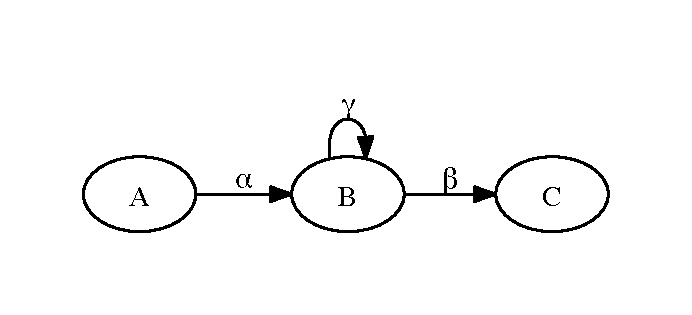
\includegraphics[trim=40 40 40 40,scale=0.6]{images/dfa_re_general}\\
$\alpha\gamma^*\beta$
\end{center}
Which means, if we were to delete state $B$ above, the our new edge from $A$ to
$C$ would be $\alpha\gamma^*\beta$. Note, if $\gamma$ is empty (there's no self loop)
then it's just $\alpha\beta$.

\begin{center}
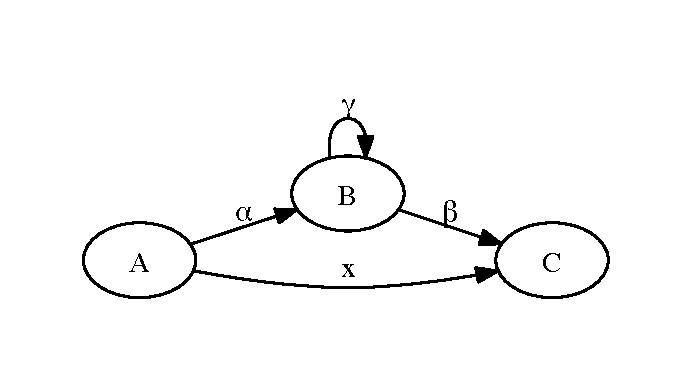
\includegraphics[trim=40 40 40 40,scale=0.6]{images/dfa_re_general2}\\
$x+(\alpha\gamma^*\beta)$
\end{center}
Which means that if we delete state $B$ above, and an edge from $A$ to $C$ exists
already, then the new edge is the union of both the general equation above,
and the existing edge.

% -! DFA minimization
%   - Table-construction algorithm
\subsection{DFA Minimization}

    \subsubsection{Table Conversion Algorithm}
    Draw a table with all states of the DFA on both the $x$ and the $y$ axis.
    Consider all input strings of length $0..n$. Start from a state $s$ on
    the $x$ axis, if an input string of length $n$ reaches a state that is final,
    and a state on the $y$ axis given the same input does not reach a final state
    (or vice versa), then we know that those states are not equal, and their cell
    can be marked off. Once a round of this goes by without any cells being
    marked, then we know that the states corresponding to cells that
    are not marked are equivalent.

    \subsubsection{Brzozowski's Algorithm}
    This algorithm is quite simple. The crux of it is that an NFA to DFA conversion
    naturally results in a minimization of the NFA. So the algorithm is as-follows:
    Take a DFA, reverse it to get an NFA, convert that NFA to a DFA again, take
    this new reversed DFA and reverse it to get the original language back, then
    convert the NFA resulting from the reversal into a DFA.


\section{Context Free Languages}
% Context-Free languages:
% - CFL formalism
% - RL and LL to NFA/DFA conversion
%   - RL conversion via reversal closures
\subsection{Closures}
Where $C$ is a context-free language, $R$ is a regular language, and $?$ is
an Unknown language.

\settowidth{\templength}{$C \cup C \spto C$}
\addtolength{\templength}{1cm}
\begin{tabular}{lp{\templength}l}
\textbf{Closed:} & & \textbf{Unclosed:} \\
$C^R \spto C$ & $C \cup C \spto C$ & $\overline{C} \spto ?$\\
$C^* \spto C$ & $C \cap R \spto C$ & $C \cap C \spto ?$\\
$CC \spto C$  & $C \cup R \spto R$ & $C \spbackslash C \spto ?$\\
$h(C) \spto C$ & & \\
\end{tabular}

% - Shortcuts for solving pumping lemmas
\subsection{Pumping Lemma}
\begin{align*}
  \exists N \in \mathbb{N}: & \\
          \forall w \in L : & |w| \geq N \impl \\
\exists uvxyz \in \Sigma^*: & \quad w = uvxyz \\
                            & \land |vy| > 0 \\
                            & \land |vxy| \leq N \\
                            & \land \forall i \geq 0: uv^ixy^iz \in L
\end{align*}

\subsection{CFG to PDA Conversion}

\subsection{Chomsky Normal Form}
\subsection{Cocke-Kasami-Younger (CKY) Parsing}

\subsection{Ambiguous Context Free Languages}
These are languages that have two separate parse-trees. To prove
that a language is ambiguous, show that it actually has two separate
parse-trees.

Example ambiguous grammar:
\[
    E \spto E + E \spbar E * E \spbar \texttt{NUMBER}
\]
% TODO: Needs graph example

\subsection{Consistency and Completeness}
\begin{description}
    \item[{\small Consistency:}] All strings generated by a grammar are 
    in the language.
    \item[{\small Completeness:}] The grammar generates all strings 
    in the language.
\end{description}

You cannot know that a grammar defines a language until you show both.
For example, if we want to define the language $\{a^nb^n | n \in \mathbb{N}\}$,
the grammar:
\[
    S \spto aabb
\]
Is \textit{consistent} because it only generates strings in the language,
but not complete because it doesn't generate all strings in the language.
Likewise, the grammar:
\[
    S \spto aS \spbar bS \spbar \varepsilon 
    \;\;\quad (\textit{grammar for }\{a, b\}^*)
\]
Is complete, it generates all possible strings in the language, but not
consistent because it generates many strings that are, in-fact, outside of
the language.


% Cardinality
% (mostly done) Schroder-Bernstein theorem
\section{Cardinality}
\subsection{Diagonalization}
Diagonalization is a general method for showing that the cardinality of
two infinite sets is not the same. So say that we have two infinite sets $A$ and $B$,
in this particular case, lets consider $B = 2^A$. Now, by definition $B$ can
be expressed as a set of infinite sets. We can begin writing out these sets,
$s_1, s_2, \ldots, s_n$. Diagonalization tells us that no matter how many
of these sets we make, there will always exists another set $s$ that has not yet
been expressed. This set $s$ is constructed by going through the list of created
sets $s_1, s_2, \ldots s_n$ and putting an element in $s$ that does not exists in
each set, this way, it cannot ever be equal to another set because it
contains at least one element that is guaranteed to not be in that set.

Note, this does not apply for non-infinite mappings. A finite number of infinite
sets can be mapped to a single infinite set using a pairing function.

\subsection{Schr\"{o}der-Bernstein Theorem}
The Schr\"{o}der-Bernstein theorem states that, for any two sets $A$ and $B$
if there exists an \textit{injective} function from $A \to B$, and
there exits an injective function from $B \to A$, then $|A| = |B|$.
Note that the injective function doesn't require every item of $A$ to map
to every item of $B$, only that every item of $A$ maps to \textit{an} item
of $B$ (and vice versa).

% Turing Machines
\section{Turing Machines}
Formaly a Turing machine is represented as tuple in the form 
$(Q, \Sigma, \Gamma, \delta, q_0, B, F)$. $Q, \Sigma, q_0$, and $F$ are the same
for PDAs and DFAs. $\Gamma$ is the tape alphabet, and since the input string
is presented on the tape, $\Sigma \subset \Gamma$ is always the case. $B$ is
the blank character. The $\delta$ is defined like so:
\[
    \delta : Q \times \Gamma \spto Q \times \Gamma \times \{L, R\}
\]
Which means the delta functions maps pairs of states an inputs, to a new state,
a value to replace the current value on the tape, and \textit{movement}. $L$ moves
the head left on the taps, and $R$ moves the head right on the tape. Since `staying-put'
can be trivially simulated $S$ is sometimes included as a movement as well. TMs
can also be non-deterministic, in that case the $\delta$ function changes to:
\[
    \delta : Q \times \Gamma \spto 2^{Q \times \Gamma \times \{L, R\}}
\]
Which allows it to be in multiple states at the same time, since it can transition
to multiple states with a single input.

\subsection{Terminology and Notation}
\begin{tabular}{rp{0.71\linewidth}}
$\langle M \rangle$ & String representation of Turing machine $M$. \\
halting & When a machine stops execution. \\
acceptance & When a machine halts in a final state. \\
rejection & When a machine halts and is not in a final state. \\
decider & A decider is a Turing machine that defines a language
          of Turing machines that conform to a yes or no question. \\
\end{tabular}

% Decidability
\section{Decidability}
\subsection{Recognizable and Enumerable}
\begin{description}
    \item[{\small Turing Recognizable (TR):}] A language $L$ where there exists some
    Turing machine $M$ that can recognize it.
    \item[{\small Recursively Enumerable (RE):}] A language $L$ where all strings in
    the language can be enumerated by some machine $M$.
\end{description}

Every language that is Turing Recognizable is also Recursively Enumerable since
an enumerator can be built from a recognizer, and a recognizer can be built
using an enumerator.

\subsection{Halting Problem}
The halting problem states building a Turing machine $P$ that can detect
whether any other Turing machine will halt is impossible. The proof is as
follows:

Assume that we have a Turing machine $P$, that when given a Turing machine
$M$ and string $w$ as input ($\langle M, w \rangle$), $P$ will (in a finite
computation time) accept in the case that $M$ halts on input 
$w$, or reject in the case that $M$ loops on input $w$. We can then
define a new Turing machine $Q$ that takes a single Turing machine $M$ 
as input. $Q$ will then ask $P$ whether machine $M$ halts when given
itself as input (does $P(\langle M, M \rangle)$ halt?). If $P$ 
accepts (says that $M$ halts) the $Q$ will loop. If $P$ rejects 
(says $M$ will loop) then $Q$ halts. Now, we can supply $Q$ as input
to machine $Q$. $Q$ will then run $P(\langle Q, Q \rangle)$. If $P$
accepts, then $Q$ will begin to loop, but $P$ said that $Q$ would
halt. This is a contraction, a general $P$ decider for the halting problem
cannot exist.

This same proof style as above can be used to perform a proof for any decider
from first principals. Just assume that the decider $P$ exists, generate a
machine $Q$ that takes a machine as input, the runs that decider on
the machine given itself as input $P(\langle M, M\rangle)$. Make machine $Q$
return the opposite of whatever $P$ says, and then pass $Q$ to $Q$. $P$ will
never be able to decide it.

\subsection{Mapping Reduction}
A mapping reduction between $A \subseteq \Sigma^*$ and 
$B \subseteq \Sigma^*$ is a function $f : \Sigma^* \to \Sigma^*$ if
$\forall x \in \Sigma^*, x \in A \Leftrightarrow f(x) \in B$. More plainly,
a function $f$ such that I can pick any $x$ in $A$, and $f(x)$ will also
be in $B$. The ``mapping reduction from $A$ to $B$'' is typically denoted
as $A \leq_m B$. A mapping reduction in polynomial time is denoted
$A \leq_p B$.

The general steps for a mapping reduction $A \leq_m B$ are as follows:
\begin{enumerate}
    \item $A$ is designated the ``known undecidable'' language.
    \item $B$ is designated the ``unknown'' language.
    \item Create a function $f$ that maps all elements of $A$ into $B$.
\end{enumerate}

To form $f$ you usually assume the decider for $B$ ($D_B$), then you construct
a machine $M$ that uses to decider $D_B$ to become a decider for $A$ ($D_A$).
For example, we can map $A_{TM}$ onto $Halt_{TM}$ using the following method:

Assume that a decider $R$ for $A_{TM}$ exists. We will now construct
a decider $S$ for $Halt_{TM}$ from $R$. $S$ has two inputs a machine $M$ and
an input string $w$. First, $S$ will run decider $R$ on $\langle M, w\rangle$,
if $R$ accepts, then $S$ accepts. If $R$ rejects, then $S$ accepts. We
now have a decider for $Halt_{TM}$ which is undecidable, a decider for
$A_{TM}$ cannot exist.

\subsection{Rice's Theorem}
``Every non-trivial partitioning of the space of Turing machine 
codes based on the languages recognized by these Turing machines 
is undecidable.''

More formally, given a property $\property$, where $\property$ is
non-trivial (not $\emptyset$ or $\Sigma^*$) the language below is
undecidable.
\[
    \{\langle M \rangle \spbar M \text{ is a Turing machine and } 
        \property(\langof(M))\}
\]

% PCP problem
\section{Post's Correspondence Problem}
Post's Correspondence Problem (PCP) is as follows. Say we have a finite set of
tuples in the form: $\{\langle x, y \rangle \spbar x, y \in \Sigma^*\}$. We can think
of these tuples like a set of blocks with a top half and a bottom half, where
the $x$ item is the top half and the $y$ item is the bottom half. Now to 
solve the PCP, find an arrangement (with possible repetitions) where the
string formed by the top blocks read left to right, is the same as the string
formed by the bottom blocks read left to right.

\subsection{Enumeration}
The set of solvable instances of this problem can be generated quite easily.
Make a machine that constantly generates two strings $w_x$ and $w_y$. A split
of $w_x$ (or $w_y$) is a set of strings that when re-ordered and concatenated forms
$w_x$ (or $w_y$). Now, make a set of all possible split of $w_x$ ($S_{w_x}$), and a set of
splits for $w_y$ ($S_{w_y}$). Then, cross every split in $S_{w_x}$  with every split
in $S_{w_y}$. Continue doing this for all possible strings 
$w_x \in \Sigma^*$, $w_y \in \Sigma^*$ where $|w_x| = |w_y|$.

\subsection{Decidability}
In the case of $|\Sigma| > 2$, the PCP is undecidable. This can be shown via
a mapping reduction that maps PCP into $A_{TM}$. The proof is rather involved, but
at a high-level, possible states of a Turing machine are expressed as PCP
pairs. A solution to the PCP problem containing these pairs is the \textit{execution
history} of the TM that accepted the string.

% NP-Completeness
\section{NP-Completeness}
\subsection{Problem Classes}
\begin{description}
    \item[{\small P:}] The set of problems that can be solved
    in polynomial time. Contained in NP.
    \item[{\small NP:}] The set of problems that can be solved
    in non-deterministic polynomial time.
    \item[{\small NP-hard:}] The set of problems that can be
    polynomial time reduced to every other problem in NP.
    \item[{\small NP-complete:}] The set of problems that are
    in both NP, and NP-hard.
\end{description}
\subsection{Proving NP-Completeness}
There are two steps to proving that a languages is in NP-complete.
First you have to show that it is NP, and then you have to show that
it is in NP-hard.

\subsubsection{Verifiers}
One way to show that a problem is in NP is by using a verifier. A verifier
is a Turing machine $V_L$ such that for all $w \in \Sigma^*$, their exists
some $c$ such that $w \in L$ when $V_L(w, c)$ accepts. Intuitively this can
be understood as ``There is a machine that can check the answers to problems
quickly''.

To give a concrete example, consider k-Clique. A verifier for k-Clique assumes
that $w$ is some graph, and $c$ is a set of nodes in graph $w$ that forms
a k-Clique. A machine that checks whether or not the set of nodes $c$ actually
forms a k-Clique is trivial and can easily be performed in a finite amount of
time.

\subsection{NP-hard Reduction}
The easiest way to show that a problem is in NP-hard, is by reducing an existing
NP-hard problem to the problem you want to prove is NP-hard using a polynomial  
mapping reduction. The classic problem to reduce from is 3-SAT.

\section{Chomsky Hierarchy}
Recursively Enumerable $\leftarrow$ 
Context-Sensitive $\leftarrow$ 
Context-Free $\leftarrow$ Regular.


\end{multicols*}
\end{document}
